%Schriftgr��e, Layout, Papierformat, Art des Dokumentes
\documentclass[12pt,oneside,a4paper]{scrartcl}
%Das Paket erzeugt ein anklickbares Verzeichnis in der PDF-Datei.
\usepackage{hyperref}

%Einstellungen der Seitenr�nder
\usepackage[left=3cm,right=4cm,top=2.5cm,bottom=2.5cm,includeheadfoot]{geometry}

%Zeilenabstand
%\renewcommand{\baselinestretch}{1.25}\normalsize %f�r 1,5 zeilig
\usepackage{setspace}

%Einr�ckung eines neuen Absatzes
\setlength{\parindent}{0em}

%neue Rechtschreibung
\usepackage[ngerman]{babel}

%Umlaute erm�glichen
\usepackage[utf8]{inputenc}

%Kopf- und Fu�zeile
\usepackage{fancyhdr}
\pagestyle{fancy}
\fancyhf{}

%Linie oben
\renewcommand{\headrulewidth}{0.5pt}

%Fu�zeile rechts bzw. au�en
\fancyfoot[C]{\thepage}
%Linie unten
\renewcommand{\footrulewidth}{0.5pt}

%Bilder einfuegen
\usepackage{graphicx}

%Code
\usepackage{listings}
%fuer fette typewriter Schrift
\renewcommand{\ttdefault}{pcr}

%Farben (benoetigt fuer listings)
\usepackage{color}
\usepackage[usenames,dvipsnames]{xcolor}

%%%%%%%%%
% Style %
%%%%%%%%%
%
% Hier ein paar Befehle und Konventionen um das Schriftbild einheitlich zu halten
%
% Bitte folgende standard Befehle nutzen:
%
% \emph{} zum Hervorheben von Text
%
% \url{} um Web-Adressen darzustellen 
%
% Codeformatierung
\newcommand{\codeformat}{\small\ttfamily}
\newcommand{\classcolor}{\color{DarkOrchid}\bfseries}
%
% vor jeder lstlisting-Umgebung aufrufen, 1. caption, 2. label
\newcommand{\javalstset}[2]{
\lstset{% general command to set parameter(s)
	basicstyle=\codeformat, % print whole listing small
	keywordstyle=\classcolor,
	% underlined bold black keywords
	identifierstyle=, % nothing happens
	commentstyle=\color{Gray}, % white comments
	stringstyle=\color{Blue}, % typewriter type for strings
	showstringspaces=false % no special string spaces 
	tabsize=3,
% ACHTUNG: lstlisting stellt Tabulatorzeichen mit dar! %
	language=Java,
	captionpos=t,
	caption={#1},
	label={#2},
	frame=trbl,
	breaklines=true,
	breakatwhitespace=true
	}
}
%
% ein einzelnes Wort in Codeformatierung darstellen
\newcommand{\code}[1]{{\codeformat{#1}}}
\newcommand{\codeclass}[1]{{\classcolor\codeformat{#1}}}
%
% Anführungszeichen
\newcommand{\gaensefuesse}[1]{"`#1"'}
%
%%%%%%%%%%
% Style/ %
%%%%%%%%%%

\begin{document}
%Beginn der Titelseite
\begin{titlepage}
\begin{small}
\vfill {Technische Universit\"at Dortmund\\ 
Fakult\"at Informatik \\
Lehrstuhl 5, Prof. Dr. Bernhard Steffen \\
Wintersemester 2012/13}
\end{small}


\begin{center}
\begin{Large}
\vfill {\textsf{\textbf{
Aktuelle Themen der Dienstleistungsinformatik\\\ \\
Projekt: Kontakte
}}}
\end{Large}
\end{center}

\begin{small}
\vfill Markus Marzotko, Thorben Seeland \&\ Dominic Wirkner\\ 
\today
\end{small}

\end{titlepage}
%Ende der Titelseite  
%Inhaltsverzeichnis (aktualisiert sich erst nach dem zweiten Setzen)
\tableofcontents
\thispagestyle{empty}
%Beginn einer neuen Seite
\clearpage
%Anderthalbzeiliger Zeilenabstand ab hier
\onehalfspacing

\section{Einleitung}
Als Abschlussübung der Vorlesung Aktuelle Themen der Dienstleistungsinformatik im Wintersemester 2012/13 an der TU-Dortmund sollten die teilnehmenden Studenten ein Projekt zum Thema Webservices durchführen. Dieser Bericht erläutert nun im Detail, wie das Projekt \textit{Kontakte} durchgeführt wurde. \\

In Kapitel 1 wird zunächst die genaue Aufgabenstellung erläutert, welche das eigentliche Projektziel darstellt. In diesem Zusammenhang werden auch erste Überlegungen zur Projektplanung und -struktur aufgeführt.\\

Daraufhin werden in Kapitel 2 die konkreten Projektbausteine behandelt. Zunächst werden die beiden Schnittstellen zu SAP und Google, welche auf Webservices basieren, im Detail erläutert, bevor es im Anschluss mit dem Thema der SIB-Programmierung weitergeht. Es wird erläutert, wie die SIB-Programmierung im Detail funktioniert und inwiefern die oben beschriebenen Schnittstellen in diesem Bereich ihre Anwendung finden.\\

Kapitel 3 beschäftigt sich mit dem konkreten Projektergebnis: dem fertigen jABC-Modell. Es wird der durch das Modell beschriebene Prozess im Detail erläutert und einige Fragen des Modelldesigns behandelt.\\

Abschliessend folgt in Kapitel 4 die konkrete Betrachtung der Projektergebnisse, um den Erfolg des Projektes zu beurteilen. 


\subsection{Projektbeschreibung}
Als Grundlage für die Aufgabenstellung diente ein fiktives Szenario in Form einer Umstellung der informationstechnischen Infrastruktur eines Unternehmens. Konkretes Thema für dieses Projekt war die Migration von kontaktbezogenen Stammdaten aus der Datenbank von SAP in das System von Google. Für die Migration mussten drei Gruppen von Kontakten behandelt werden: Kunden, Lieferanten und Angestellte.\\
Die Migration selbst sollte dabei nicht der trivialen Strategie folgen, alle vorhandenen Kontakte in einem Prozess komplett zu kopieren. Aufgrund der Existenz von sogenannten "'Karteileichen"` in der Datenbank von SAP, wurde eine Strategie vorgegeben, welche eine Migration nur bei Bedarf vorsieht. Dadurch wird garantiert, dass das System von Google nur Kontaktdaten enthält, welche aktiv von dem Unternehmen genutzt werden.\\
Die Migrationsstrategie behandelt demnach nur einen einzelnen Kontakt und gliedert sich in drei Teile. Zunächst muss im System von Google überprüft werden, ob der gewünschte Kontakt schon migriert worden ist. Ist dies der Fall, so ist findet keine erneute Migration statt und der Prozess ist beendet.\\
Falls der gesuchte Kontakt nicht im System von Google existiert, wird versucht, diesen in der Datenbank von SAP zu finden und im Anschluss nach Google zu übertragen. Da es bei einer Suche nach einem Kontakt, abhängig von den Kriterien, sowohl bei Google als auch bei SAP dazu kommen kann, dass mehrere Ergenisse zurückgeliefert werden, muss es dem Nutzer möglich sein, den gewünschten Kontakt aus dieser Ergebnisliste manuell auszuwählen. In diesem Fall endet der Prozess mit einer erfolgreichen Migration von SAP nach Google.\\
Zudem muss die Tatsache abgedeckt sein, dass der gesuchte Kontakt ein gänzlich neuer ist, welcher bisher noch in keiner Datenbank auftaucht. Dann soll der Kontakt nach manueller Dateneingabe bei Google angelegt werden.

\subsection{Erste Überlegungen}
Damit eine effiziente Projektplanung gewährleistet werden kann, muss zunächst die Aufgabenstellung analysiert werden. Das Ziel dieser Analyse ist es zunächst, Bereiche zu identifizieren, welche unabhängig bearbeitet werden könne. Dies unterstützt die Aufgabenverteilung an die einzelnen Projektmitglieder und legt deren Verantwortungsbereiche fest.\\
Da diese Teilbereiche im Projektzusammenhang jedoch an einigen Stellen miteinander interagieren sollen, müssen zudem geeignete Schnittstellen an den Berührungspunkten definiert werden.\\
Zudem gilt es auch, sich am Anfang der Planung über einzusetzende Technologien zu einigen, welche die Entwicklung unterstützen.

\subsubsection{Projektstruktur}
Aufgrund der Aufgabenstellung lassen sich leicht folgende zwei unabhängige Bereiche identifizieren: die beiden Schnittstellen zu den Datanbanksystemen. 

- Analyse der Projektstruktur / Identifikation von autonomen Mechanismen:
	- zur Aufgabenverteilung an einzelne Mitglieder: Spezialisten schaffen, Verantwortungsbereiche festlegen
	- Identifikation von Berührungspunkten der Teilbereiche
	- Aufteilung des Projektes (siehe Grafik)
	
\subsubsection{Das Kontakt-Objekt als Schnittstelle}
- Das Kontakt Objekt:
	- Bildung einer repräsentativen Schnittmenge von typischen Kontaktattributen
		- Wahl der Attribute
		- ID-Speicherung für Möglichkeit der Anwendung von komplexeren Migrations-Strategien
	- Modellierung einer allgemeinen Klasse Kontakt als Schnittstellenobjekt
		- zwischen den Funktionen, innerhalb des jABC-Modells
		
\subsubsection{Eingesetzte Technologien}
- Verteilte Programmierung -> VCS git
- verwendete Sprache Java -> JUnit-Tests zur Verifikation der Schnittstelle zw. SIBs und Konnektoren
- Apache-Maven im Hinblick auf Unterstützung von build und deploy Aufgaben
	- autom. Tests im build
	- unterstützung beim deploy durch erzeugung eines jar-Archivs inkl. notwendiger Abhängigkeiten
		- eingentlich Bad Practice
		- Im Umgang mit jABC simpler


\section{Unsere Projektbausteine}
 - Im Folgenden Beschreibung, besondere Überlegungen und Probleme(!)/Entscheidungen der einzelnen Elemente





\subsection{SAP-Connector}
\subsubsection{Aufgabe des SAP Connectors}

Die Aufgabe des SAP Connectors besteht darin, die Datenbank im ES Workplace nach einem 
gegebenen Filter zu durchsuchen. Die gefilterten Datensätze werden zurückgegeben. 

\subsubsection{Aufbau und Programmablauf}

Alle Operationen dienen dazu, Datensätze aus den Datenbanken des ES Workplace auszulesen. Der ES Workplace stellt hierfür 
eine Datenbank mit Testdatensätzen bereit, sowie die erforderlichen Webservices, um eine Verbindung zur Datenbank, 
die Authentifizierung und die Suche selbst durchzuführen. Die erforderlichen Webservices liegen als XML Dateien vor, werden 
jedoch zur Verwendung in SIBs als Java Klassen benötigt. Dafür wird Java API for XML Web Services verwendet, welches seit
Version 1.6  Bestandteil der Java SE ist. Mittels Jax-WS können in der Konsole durch einen wsimport Befehl alle benötigten 
Webservices von XML Dateien in Java Klassen umgewandelt werden. 
\ \\
Der SAP Connektor erhält ein Objekt vom Typ Contact. Dieses Objekt enthält die vom Benutzer geforderten Filtereinstellungen 
betreffend Vorname, Nachname, Postleitzahl, Stadt, Straße und Firma. Außerdem wird der Typ nach Kunde, Lieferant und 
Mitarbeiter unterschieden. Dieses Objekt wird verwendet, um in der Datenbank des ES Workplace, nach dem entsprechenden Typ,
Datensätze zu filtern. In Abhängigkeit von der Typbestimmung werden unterschiedliche Webservices ausgeführt:
\ \\

\textbf{Lieferant}
\begin{itemize}
\item Find Supplier by Name and Address
\item Read Supplier Basic Data 
\end{itemize}

\textbf{Mitarbeiter}
\begin{itemize}
\item Find Employee by Elements
\item Find Employee Address by Employee
\end{itemize}

\textbf{Kunde}
\begin{itemize}
\item Find Customer by Elements
\end{itemize}

\ \\
Zunächst soll hier das Programm am Beispiel des Kundenwebservices beschrieben werden. Anschließend werden die Besonderheiten
bei den Webservices für Mitarbeiter und Lieferant erläutert.

\ \\

Zunächst müssen die notwendigen Objekte der Klassen des Webservices ``Find Customer by Elements'' erstellt werden. Mittels
einer Klasse die immer mit dem Schlüsselwort SERVICE beginnt, kann ein Objekt erzeugt werden auf dem eine getBinding Methode
ausgeführt wird. Das erstellte Verbindungsobjekt wird dann zu einem Objekt vom Typ Binding Provider gecastet, auf welchem dann
mittels getRequestContext() Methoden Passwort und Username gesetzt werden können. Für die Authentifizierung ist normalerweise
auch noch eine Webadresse anzugeben, allerdings ist hier die Adresse der Testdatenbank bereits enthalten. Das 
Verbindungsobjekt verfügt über eine einzige Methode, die ein Objekt mit Suchkriterien übergeben bekommt und eine Liste 
von Suchergebnissen zurückliefert. Die Suchkriterien können mit einfachen bereits integrierten set Methoden gesetzt werden,
die Suchergebnisse über get Methoden ausgelesen werden. Anschließend werden die Suchergebnisse als Liste von Kontaktobjekten
zurückgegeben.





\subsubsection{Probleme}

\subsubsection{Ausblick}

\subsection{Google-Connector}
\subsubsection{Die Bibliothek \emph{gdata}}
Die Google-Bibliothek \emph{gdata} ist eine frei verf\"ugbare Bibliothek zum erstellen von
 Clientapplications für die Services der Google-Cloud.
\emph{gdata} kapselt die Webservices komplett in Java-Klassen, so dass ein importieren
 (z.\ B.\ mit \emph{wsimport}) nicht mehr notwendig ist.

\subsubsection{Authentifizieren und Verbinden mit \emph{gdata}}
Google bietet zwei Authentifizierungsverfahren an
\begin{enumerate}
	\item\emph{OAuth}
	\item Username und Passwort
\end{enumerate}
\emph{OAuth} ist ein Service, der bei erfolgreicher Anmeldung ein Token erstellt, mit dem
 der Client von Google bereitgestellte Services aufrufen und sich authentifizieren kann.
So muss der Client die Anmelde-Daten des Nutzers nicht speichern, sondern nur den Token.
In Abbildung \ref{fig:google_oauth} wird ein Beispiel f\"ur die Nutzung von \emph{OAuth} dargestellt.
% TODO Quelle https://developers.google.com/accounts/docs/OAuth2
\begin{figure}[h!]
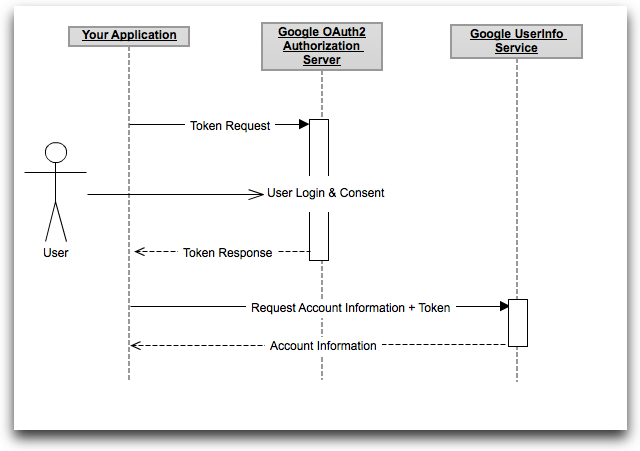
\includegraphics[width=\textwidth]{Bilder/googleOauth.png}
\label{fig:google_oauth}
\caption{Nutzungsbeispiel f\"ur \emph{OAuth}}
\end{figure}

Da wir unseren eigenen Account nutzen und die Daten nicht Sicherheitskritisch sind, haben
 wir die zweite Variante gew\"ahlt und authentifizieren uns bei jedem Service-Aufruf mit
 Username und Passwort.

\subsubsection{Kontakte suchen}
Die \emph{gdata}-Bibliothek bietet die Möglichkeit, Kontakte mit Angabe eines \emph{Querys}
 herunterzuladen.
Das \emph{Query} kann jedoch nur zwischen Gruppen unterscheiden, jedoch nicht nach anderen
 Kriterien wie z.\ B.\ dem Vornamen oder dem Nachnamen eines Kontakts filtern.

Das Suchen von Kontakten geschieht in unserem Projekt durch das Herunterladen aller Kontakte
 einer Gruppe und anschließendem sortieren "`von Hand"'.

\subsubsection{Kontakte einf\"ugen}
Das Einfügen von Kontakten ist über ein erstelltes Service-Objekt 



\subsection{SIB-Programmierung}

In diesem Kapitel wird die SIB-Programmierung eingegangen. Dabei wird zunächst auf die Implementierung von SIBs im allgemeinen eingegangen. Darauf folgt die genaue Beschreibung der für das Projekt erstellten SIBs, sowie die Darstellung zweier Besonderheiten im diesem Entwicklungsprozess.

\subsubsection{Allgemeines zur SIB-Programmierung}
Im jABC können SIBs über eine Baumstruktur ausgewählt und dann bequem in das Prozessmodell eingebunden werden. Um die verwendeten SIBs miteinander zu verbinden, besitzt jedes SIB fest definierte ausgehende Kanten, im jABC-Kontext auch Branches genannt. Zudem ist es üblich, dass ein SIB definerte Parameter benötigt, um dessen Ausführung zu steuern. Je nach Zweck des einzelnen SIB unterscheiden sich daher desser Branches und Parameter. Im folgenden wird nun erläutert, wie ein solches SIB erstellt wird.\\

Da jABC eine Java-Anwendung ist und die Ausführung des Prozessmodells, und dadurch auch die Ausführung der einzelnen SIBs an sich, innerhalb von jABC stattfindet, werden die einzelnen SIBs ebenfalls in Java implementiert. Ein SIB wird dabei durch eine Java-Klasse repräsentiert, welche mit der Annotation @SIBClass versehen ist. Durch diese Annotation wird die Java-Klasse von jABC als SIB erkannt.\\

Damit das SIB innerhalb einer Modellausführung verwendet werden kann, müssen jedoch zunächst noch Branches und Parameter definiert werden. Mögliche Branches werden dabei über eine öffentliche Klassenvariable namens BRANCHES definiert, welche vom Typ Strings[] ist. Auch SIB-Parameter sind öffentliche Klassenvariablen. Der Name der Variablen ist beliebig und es kann aus den üblichen Standard-Typen (z.B. boolean, int, String, ...) ausgewählt werden. Für die Notwendigkeit der Anwendung von komplizierteren Parametern, wie ganzen Klassen, stellt jABC den Variablentyp ContextKey zur Verfügung. Mit diesem ist es möglich Objekte innerhalb des Ausführungskontextes von jABC zu referenzieren. Diese können dann lesend wie schreibend verwendet werden. In jABC ist der Ausführungskontext über eine map realisiert. Daher auch der Name ContextKey des Variablentyps, denn bei der Deklaration einer Variable von diesem Typ ist lediglich der zugehörige Schlüssel aus der map anzugeben. Die Klassenvariable kann dann dazu verwendet werden, auf die Daten im Ausführungskontext zuzugreifen. \\

Jedoch bedarf es noch einer weiteren Ergänzung, um ein SIB vollständig zu implementieren. Es muss noch definiert werden, was dieses SIB eigentlich tun soll. Hierfür muss die Java-Klasse des SIBs das Interface Executable implementieren, welches verlangt, dass die Klasse die Methode trace() definiert. Diese Methode trace() wird innerhalb von jABC in dem Moment aufgerufen, wenn die Ausführung des SIBs beginnen soll. Als Parameter wird eine Variable vom Typ ExecutionEnvironment übergeben, welche für den Zugriff auf den Ausführungskontext erforderlich ist. Zuletzt muss jABC noch mitgeteilt werden, welcher Branch im Anschluss an die Ausführung gewählt werden soll. Die Methode trace() besitzt hierzu den Rückgabewert String. Überlicherweise wird der Rückgabewert aus dem wie oben definierten String-Array BRANCHES ausgewählt.\\

Das folgende Listing zeigt exemplarisch den Kopf einer typischen Implementierung einer SIB-Klasse.

% Listing SIB-Klasse %

@SIBClass("My-SIB")
public class MySib implements Executable {

	// Branches
    public final String[] BRANCHES = {"default", "error"};

    // Parameter
    public ContextKey someKey = new ContextKey("someKey");
    public String title = "Nice Title";

    @Override
    public String trace(ExecutionEnvironment env) {
        ...
		return "default";
    }
	...
}	

% Listing SIB-Klasse ENDE %

\subsubsection{Spezifiktion notwendiger SIBs}
Wie bereits aus der Projektstruktur in Abbildung X ersichtlich, sind verschiedene Arten von SIBs für ein geeignetes Modell notwendig. Zum einen werden SIBs benötigt, welche die Funktionen der Konnektoren benutzen. Zum anderen müssen SIBs implementiert werden, welche über GUI-Elemente die Eingaben des Nutzers abfragen. Daraus ergibt sich die Notwendigkeit folgender SIBs.\\

Ein zentrales Element des Prozessen ist die Suche nach Kontakten anhand gegebener Kriterien. Daher werden für die beiden Suchfunktionen (bei SAP und Google) passend zwei SIBs implementiert. Die beiden SIBs unterscheiden sich jedoch nur in der Form, dass sie bei der Ausführung die jeweils passende Suchmethode der externen Datenbank verwenden. Äußerlich unterscheiden sich diese bis auf den Namen daher nicht. Als Eingabe erwarten beide Suchfunktionen einen Parameter vom Typ des oben in der Einleitung beschriebenen Kontaktobjektes. Zurück liefern dann beide Funktionen eine Liste von eben genannten Kontaktobjekten. Parameter und Rückgabewert sind als SIB-Parameter vom Typ ContextKey implementiert, wodurch eine weitere Verwendung möglich wird. Definierte Branches der beiden SIBs sind found (für den Fall dass die zurückgelieferte Liste nicht leer ist), not found (im Falle einer leeren Rückgabeliste) und error (wird gewählt, wenn die Ausführung der Suchfunktion eine Exception wift).\\

Ein weiteres Element einer Datenmigration ist das Hinzufügen der Objekte auf dem Zielsystem. Zu diesem Zweck muss ein SIB erzeugt werden, welches die passende Funktion nutzt, um Kontakte dem Google-System hinzu zufügen. Der Parameter des SIB ist in diesem Fall vom Typ ContextKey und verweist auf ein Kontaktobjekt, dessen Variablen mit passenden Werten belegt sind. Ein spezieller Rückgabewert ist in diesem Fall unnötig, denn Erfolg oder Misserfolg der Funktionsausführung wird über den gewählten Branch kommuniziert. Zu diesem Zweck besitzt das SIB die zwei Branches default (falls kein Fehler auftritt) und error (falls Exception geworfen wird, s.o.).\\

Damit ist die Kommunikation zu den externen Datenbanken ausreichen spezifiziert und es folgt die Definition der SIBs, welche für die Nutzereingaben verantwortlich sind.\\

Damit der Nutzer eine Suchanfrage definieren kann, muss jener die Daten eingeben können. Hierzu wird ein SIB generiert, welches ein Fenster (Swing-Frame) öffnet und anschließend auf die Eingabe des Nutzers wartet. Die Eingabefelder können mit den Werten eines Kontaktobjektes vorbelegt werden. Wenn die Eingabe beendet ist, speichert das SIB die Daten in den Ausführungskontext. Zu diesem Zweck wurde ein passender SIB-Parameter vom Typ ContextKey definiert. Dieser dient sowohl für die Vorbelegung als auch zur Speicherung der Eingaben. Um die Wiederverwendbarkeit zu ermöglichen, wurde das SIB um weitere Parameter erweitert. Zum einen besitzt das Kontaktobjekt eine Funktion namens validate(), mit Hilfe derer sich die Eingaben des Nutzers kontrollieren lassen. Diese kann mittels eines Parameters vom Typ boolean an- bzw. ausgeschaltet werden. Auf diese Weise ist es möglich das SIB sowohl für die Suchanfrage (keine Validierung notwendig) als auch zur Dateneingabe eines neuen Kontaktes (Validierung notwendig) zu verwenden. Zudem wurden die Branches ok (Eingabe beendet), cancel (Eingabe abgebrochen) und error (s.o.) definiert.\\

Abbildung Edit

Zuletzt fehlt noch die Möglichkeit, dass der Nutzer einen Kontakt aus einer Liste von Kontakten auswählen kann, sprich auf das Ergebnis einer Suchanfrage reagieren kann. Das hier zu implementierende SIB benötigt also einen Parameter in Form einer Liste von Kontaktobjekten. Auf der anderen Seite muss das Kontaktobjekt zurückgeliefert werden, welches der Nutzer ausgewählt hat. Ähnlich zu vorherigen SIBs, sind diese Parameter als ContextKey realisiert. Das SIB liest die Kontaktliste aus dem Ausführungskontext und befüllt ein entsprechendes Fenster. Nachdem der Nutzer einen Kontakt ausgewählt hat, werden die Daten entsprechend in den Kontext geschrieben. Es wurden die Branches ok (Eingabe beendet), cancel (Eingabe abgebrochen) und error (s.o.) definiert.\\

Abbildung Choose

Um der Konvention von jABC zu folgen wurde noch ein weiteres SIB implemtiert. In jABC ist es üblich ein sogenanntes Put-SIB zu verwenden, wenn eine Variable eines bestimmten Typs im Ausführungskontext erzeugt wird. Zu diesem Zweck startet das Prozessmodell mit einem SIB namens PutContact. Es erzeugt eine Instanz der Kontaktklasse im Ausführungskontext, welche im Verlauf der Modellausführung verändert wird, bis ihr Inhalt zum Schluss dem Google-System hinzugefügt wird.
	

\subsubsection{Besonderheit der GUI-SIBs}
Eine Besonderheit bei der Implementierung von SIBs ist die Benutzung von Komponenten des Swing-Frameworks. Üblicherweise werden die erzeugten Fenster in einem separaten Thread gestartet, was den Effekt zur Folge hat, dass nach Erzeugung des Fensters die trace()-Methode nicht auf Eingaben wartet, sondern weiter ausgeführt wird. Während der Nutzer seine Eingabe noch nicht einmal begonnen hat, ist jABC mit der Ausführung der trace()-Methode schon fertig.\\

Als Lösung des Problems bot sich die Java-eigene Möglichkeit zur Thread-Synchronisation mittels eines synchronized-Blockes an. Eine exemplarische Verwendung zeigt das folgende Listing.

% synchro listing %

In diesem Listing ist der synchronized-Blcok der trace()-Methode zu sehen. Nachdem der Swing-Frame erzeugt wurde, dient jener als Synchronisationsobjekt. Nachdem der synchronized-Block betreten wurde, wird in trace() die Methode wait() aufgerufen. An dieser Stelle stoppt die Ausführung von trace(), bis das entsprechende Gegenstück, die Methode notify(), auf dem Synchronisationsobjekt aufgerufen wurde. Dies geschieht innerhalb der ActionListener der verwendeten Buttons. Wenn der Nutzer mit der Eingabe der Daten oder der Auswahl des Kontaktes fertig ist, signalisiert er dies mit einem Klick auf einen Button. Es wird der entsprechende ActionListener des Buttons aufgerufen, welcher wiederum innerhalb eines synchronized-Block die Methode notify() aufruft und anschliessend das Fenster schliesst.\\

Die wartende trace()-Methode wird daraufhin weiter ausgeführt und kann über geeignete Klassenvariablen des Frame-Objektes die Eingaben des Nutzers abfragen und in den Ausführungskontext schreiben.

\subsubsection{die JAVA-Laufzeitumgebung in jABC}	
Eine weitere Besonderheit hat sich während des Projektes zufällig ergeben. Um das Zusammenspiel von Konnektoren und GUI-Elementen effizient zu testen, wurde auf die Ausführung der Komponenten im jABC zunächst verzichtet. Erst zum Ende des Projektes wurden die Komponenten mittels ihrer zugehörigen SIBs in jABC getestet. Es zeigte sich ein Fehler während der Ausführung, welcher ausserhalb von jABC nicht autrat. Die geworfene Exception lies darauf vermuten, dass bestimmte Bibliotheken innerhalb der Ausführung von jABC nicht gefunden werden konnten. Unter Verwendung des selben Quellcodes ausserhalb von jABC zeigte sich dieser Fehler jedoch nicht.\\
Dies legt die Vermutung nahe, dass die zur Laufzeit existierende Java-Umgebung in Form der Java-Virtual-Maschine (JVM) in beiden Szenarien nicht gleich ist. Einige Bibliotheken werden innerhalb von jABC unter anderen Paketpfaden referenziert, als es ausserhalb der Fall ist. Zu diesem Zweck mussten die Eigenschaften der JVM im jABC manuell verändert werden. Dies ist in folgendem Listing zu sehen.\\

% Listing system.setproperty %

Auch wenn die Veränderung der Laufzeit-Eigenschaften das Problem behoben haben, so ist doch generell von dieser Praxis abzuraten. Denn die veränderten Eigenschaften bleiben auch noch nach der Modellausführung im jABC bestehen, da jABC selbst ein Java-Programm ist und zur Ausführung von Modell die JVM des Programms verwendet wird. Die Ausführung anderer Modelle im Anschluss an jenes dieses Projektes kann also beeinträchtigt oder im schlimmsten Fall gar nicht erst möglich sein.




\section{Der fertige Prozess im jABC}
Abschließend fließen nun die einzelnen Komponenten, welche durch entsprechende SIBs repräsentiert werden, in das Prozessmodell ein. Die folgende Abbildung \ref{fig:jabcmodel} zeigt das fertige Projektergebnis, welches die in Kapitel \ref{sec:einleitung} beschriebene Aufgabenstellung erfüllt.

\begin{figure}[h!t]
\begin{center}
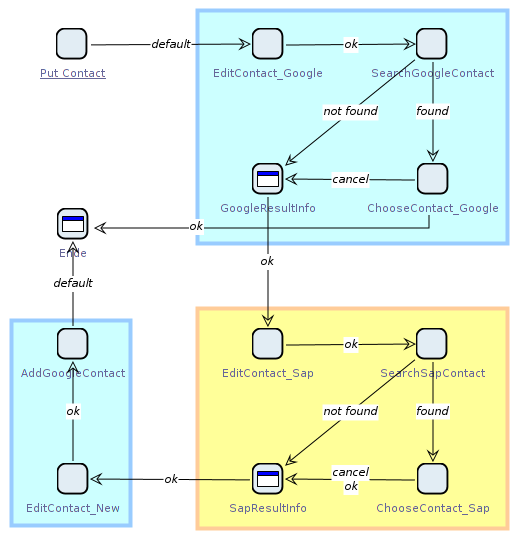
\includegraphics[width=0.65\textwidth]{Bilder/jabc_Model.png}
\end{center}
\caption{fertiges Prozessmodell im jABC}
\label{fig:jabcmodel} 
\end{figure} 

Zunächst lassen sich die farblich-gekennzeichneten Bereiche erkennen. Die blauen Bereiche enthalten die Kommunikation mit der Datenbank bei Google, während der gelbe Bereich die Kommunikation mit dem SAP-System repräsentiert. Die farbige Kennzeichnung dient auch der Tatsache, dass sich diese Bereiche in Untermodelle auslagern lassen, um diese z.B. in anderen Modellen wiederzuverwenden. Im Rahmen dieses Projektes wurde jedoch aus Gründen der Übersichtlichkeit darauf verzichtet. Ebenso verhält es sich mit den in Kapitel \ref{sec:sibs_spez} beschriebenen \textit{error}-Branches.

Zudem ist die Wiederverwendung der SIBs erkennbar, welche für die Nutzereingabe verantwortlich sind und es fällt auf, dass die Teilgraphen der Suchanfragen bei SAP und Google eine gemeinsame Struktur haben.







\section{Beurteilung des Projektes}
\label{sec:beurteilung}

Zusammenfassend lässt sich das Projektergebnis als Erfolg verzeichnen. Zum einen natürlich, weil das erzeugte jABC-Modell den Anforderungen der Aufgabenstellung genügt. Der Großteil des Erfolges ist jedoch sicherlich der Erfahrung geschuldet, welche während des Projektes gesammelt werden konnte. So zeigten sich während der Bearbeitung die Besonderheiten einer Datenmigration in Zusammenhang mit der Verwendung von Webservices. 

So muss zum einen darauf geachtet werden, ob gewählte Webservices überhaupt die Methoden zu Verfügung stellen, welche für die Aufgabenstellung benötigt werden. Während es in diesem Fall zum Beispiel möglich war bei SAP nach einzelnen Attributen von Personen zu suchen, bot der Webservice von Google diese Möglichkeit nicht. Hier mussten bei jeder Anfrage alle Kontakte zurück"=geliefert werden. Ein Aussortieren fand erst im Anschluss lokal statt.

Zum anderen ist darauf zu achten, dass im Zielsystem auch alle Attribute des Quellsystems gespeichert werden können. Unbedingt muss in diesem Zusammenhang auch darauf geachtet werden, eine ausreichende Zuordnung der Attribute des Quell- und Zielsystems zu spezifizieren. In einigen Fällen kann es daher vorkommen, dass sich bestimmte Informationen bei einer Migration nicht übertragen lassen. Im speziellen Fall dieses Projektes gab es hinsichtlich dieses Aspektes keine Probleme.

Nicht zuletzt kann das Projekt auch hinsichtlich der Zusammenarbeit der Projektteilnehmer als Erfolg verzeichnet werden. 





\clearpage
\section{Literaturverweise}
	\begin{thebibliography}{mustermarke}
	
		\bibitem{WF95} Wasserman, Stanley und Katherine Faust; \textit{Social Network Analysis: Methods and Applications}; Cambridge University Press, New York; 1995
	
		\bibitem{CLRS01} Cormen, Thomas H., Charles E. Leiserson, Ronald L. Rivest und Clifford Stein; \textit{Introduction to Algorithms, Second Edition}; The MIT Press and McGraw-Hill Book Company; 2001
		
			\bibitem{JKL04} Jacob, Riko, Dirk Kosch�tzki, Katharina Anna Lehmann, Leon Peeters und Dagmar Tenfelde-Podehl; \textit{Algorithms for Centrality Indices};\\
		In: Brandes, Ulrik und Thomas Erlebach
	
		\bibitem{BE05} Brandes, Ulrik und Thomas Erlebach; \textit{Network Analysis: Methodological Foundations}; Band 3418 der Reihe \textit{Lecture Notes in Computer Science}; Springer; 2005
	
	\end{thebibliography}
\end{document}
